\documentclass[12pt]{article} 
\usepackage[left=2.5cm, right=2cm, top=2cm, bottom=2cm]{geometry} 
\usepackage{graphicx}
\usepackage[pages=some]{background}
\usepackage{titling}
\usepackage{tabularx}
\usepackage{tikz}
\usepackage{subfigure}
\usepackage{textcase}
\usepackage{newtxtext}
\usepackage{enumitem}
\usepackage{fancyhdr}
\usepackage{graphicx}
\usepackage{multicol}
\usepackage{float}
\usepackage{tabularx}
\usepackage{adjustbox}
\usepackage{float}
\usepackage{amssymb}
\usepackage{amsmath}

\pagestyle{fancy}
\fancyhf{} 
\renewcommand{\headrulewidth}{0pt} 
\rhead{\#1810009}

\begin{document}


  \subsection*{Experiment no: 5}
  \subsubsection*{Experiment Name: STUDY OF GAS ENGINE OF BUET POWER PLANT} 
  \vspace*{0.3cm}
  \subsection*{Objectives:}
  The Key objectives of this experiment are:
  \begin{enumerate}[label=(\roman*)]
    \begin{multicols}{2}
      \item IC Engine Specification
      \item Engine Mounting 
      \item Starting System
      \item Air Intake System 
      \item Fuel Supply Unit 
      \item Ignition System
      \item Cooling System
      \item Lubrication System
      \item Exhaust System
      \item Engine Control System
      \item Engine Protection System 
      \item Engine Governing 
    \end{multicols}
    \end{enumerate}

    \subsubsection*{Engine Name Plate Data:}
      Caterpiller \\
      Gas Generator Set G3516 \\
      LEAN BURN Gas Engine \\
      Low Energy Gas Continuous 1020 \\ 
      CKW 1287 kVA \\
      50 HZ 1500 rpm 400 volts \\

    \subsection*{Engine Specification for 1 MW Engine}
    CAT LEAN BURN GAS ENGINE: \\
    G3516 LE SCAC 4 STROKE CYCLE SPARK IGNITED ENGINE  
    \begin{table}[ht]
      \centering
      \begin{adjustbox}{width=\textwidth}
      \begin{tabularx}{\linewidth}{p{0.5\linewidth} p{0.5\linewidth}}
        \hline 
        \\
        Number of Cylinders & V16 \\
        Bore, mm (in) & 170 (6-7) \\
        Stroke, mm (in) & 190 (7-5) \\
        Displacement, L & 69 (4210) \\
        Compression Ratio & 11:1 \\
        Cylinders and arrangement & 65 degree V-16 \\
        Rotation (flywheel end) & Counterclockwise rotation is standard \\
        Inlet Valve Lash & 0.51 mm (0.02 inch) \\
        Exhaust Valve Lash & 1.27 mm (0.05 inch) \\
        Firing Order (Standard) & 1-2-5-6-3-4-9-10-15-16-11-12-13-14-9-8 \\
        Firing Order (Optional) & 1-6-5-4-3-10-9-16-15-12-11-14-13-8-7-2 \\
        \\
        \hline
      \end{tabularx}
      \end{adjustbox}
      \caption{Engine Specification for 1 MW Engine}
      \label{tab:Roof}
      \end{table}

      \subsection*{Generator Specifcation}
      CAT SR4B GENERATOR \\
      \begin{table}[ht]
        \centering
        \begin{adjustbox}{width=\textwidth}
        \begin{tabularx}{\linewidth}{p{0.5\linewidth} p{0.5\linewidth}}
          \hline 
          \\
          Frame Size & 697 \\
          Excitation & Permanent Magnet \\
          Construction & Star-Delta \\
          Pitch & 0.7333 \\
          Number of Poles & 4 \\
          Number of bearings & 1 \\
          Number of leads & 6 \\
          IP Rating & Dip Proof IP22 \\
          Alignment & Pitot Shaft \\
          Lever speed capability & 125\%\\
          Wave form deviation line to line, no lead & less than 3\% \\
          Voltage Regulator & CDVR \\
          Voltage Level Alignment & +/- 5.0\% \\ 
          Voltage Regulation Steady State & +/- 5.0\% \\ 
          Voltage Regulation with 3\% speed change & +/- 5.0\% \\ 
          Telephone influence factor & less than 50 \\ 
          \\
          \hline
        \end{tabularx}
        \end{adjustbox}
        \caption{Engine Specification for Generator}
        
        \end{table}

  \vspace*{0.3cm}

        \subsection*{Engine Mounting}
        \begin{table}[ht]
          \centering
          \begin{adjustbox}{width=\textwidth}
          \begin{tabularx}{\linewidth}{p{0.3\linewidth} p{0.7\linewidth}}
            \hline 
            \\
            Standard & 330 mm, industrial type rail, engine generation mounting \\
            Optional & Spring type vibration isolators, Rubber type \\
            Function & To damper vibration generated by the engine \\
            \\
            \hline
          \end{tabularx}
          \end{adjustbox}
          \end{table}

        \subsection*{Starting System}
        \begin{multicols}{2}
          \begin{center}
            
            \begin{enumerate}
              \item Air Intake System 
              \item Air Pressure Regulator 
              \item Air Silencer 
              \item Electric Air Start Controls 
              \item Electric Starting Motors - Dual 24 Volt 
              \item Starting Aids 
              \item Battery Sets [24 volt dry], Cables and Rack  
            \end{enumerate}
          \end{center}
          \end{multicols}

          \begin{figure}[H]
            \begin{center}
              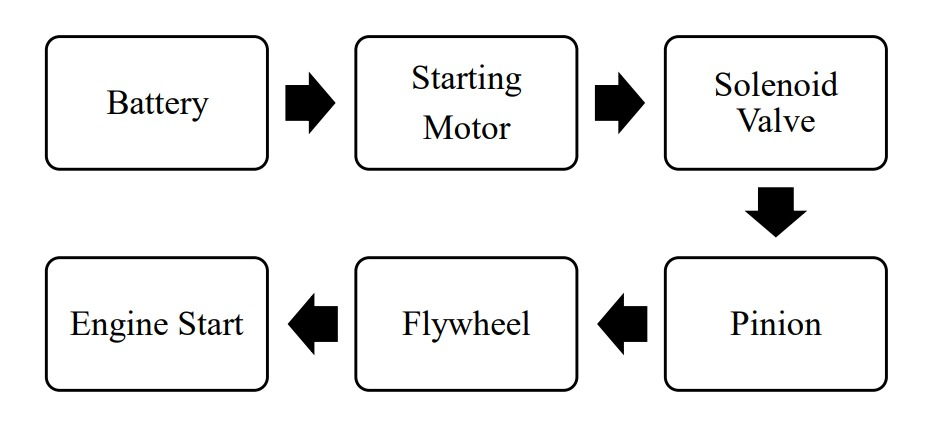
\includegraphics[width=0.7\linewidth]{img/starting_system.jpeg}
              \caption{Starting System}
            \end{center}
          \end{figure}

          \vspace*{0.6cm}
          \subsection*{Air Intake System}
          The air intake system filters the intake air to ensure fresh air charge into the engine every cycle. It consists of the following components:
          \begin{itemize}
            \item Air Cleaner - intermediate duty with service indicator
            \item Remote Air Inlet Adapters 
            \item Pre-cleaner 
          \end{itemize}

          \begin{figure}[H]
            \begin{center}
              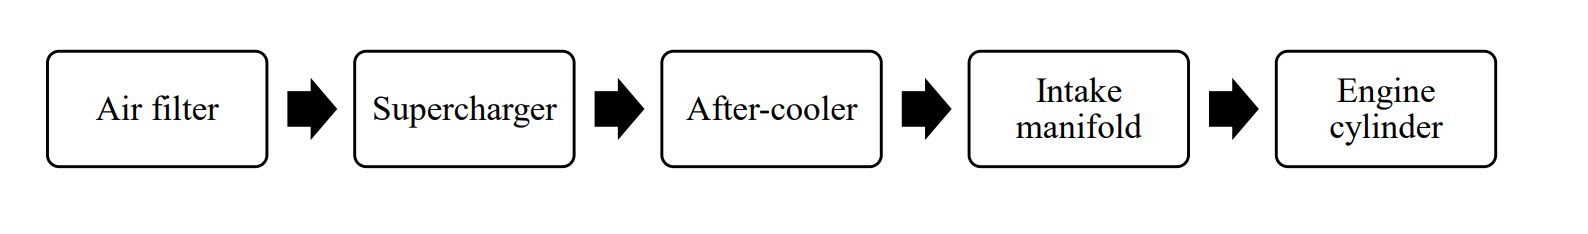
\includegraphics[width=0.98\linewidth]{img/intake_system.jpeg}
              \caption{Air Intake System}
            \end{center}
          \end{figure}

          \subsection*{Fuel Supply System}
          The fuel supply system provides a continuous supply of clean fuel to the engine. It consists of the following components:
          \begin{itemize}
            \item Gas Pressure Regulators 
            \item Natural Gas Regulator 
            \item Fuel Filter 
            \item Propane gas valve and jet kits 
          \end{itemize}
          \begin{figure}[H]
            \begin{center}
              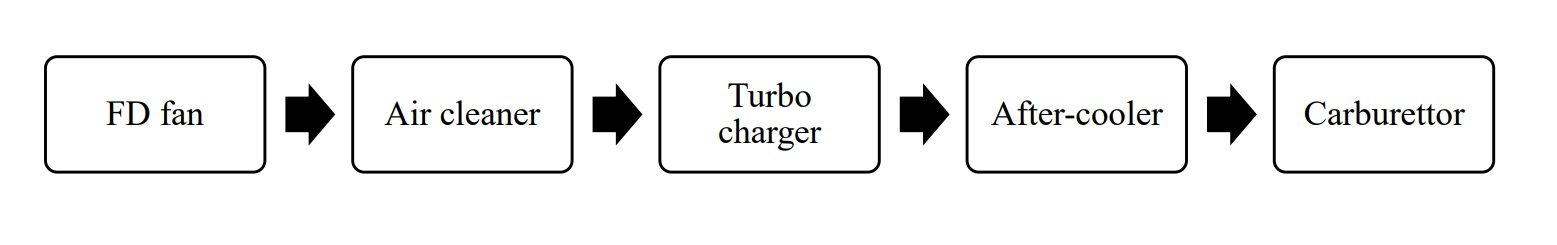
\includegraphics[width=0.98\linewidth]{img/air_supply.jpeg}
              \caption{Air Supply System}
            \end{center}
          \end{figure}
          
          \begin{figure}[H]
            \begin{center}
              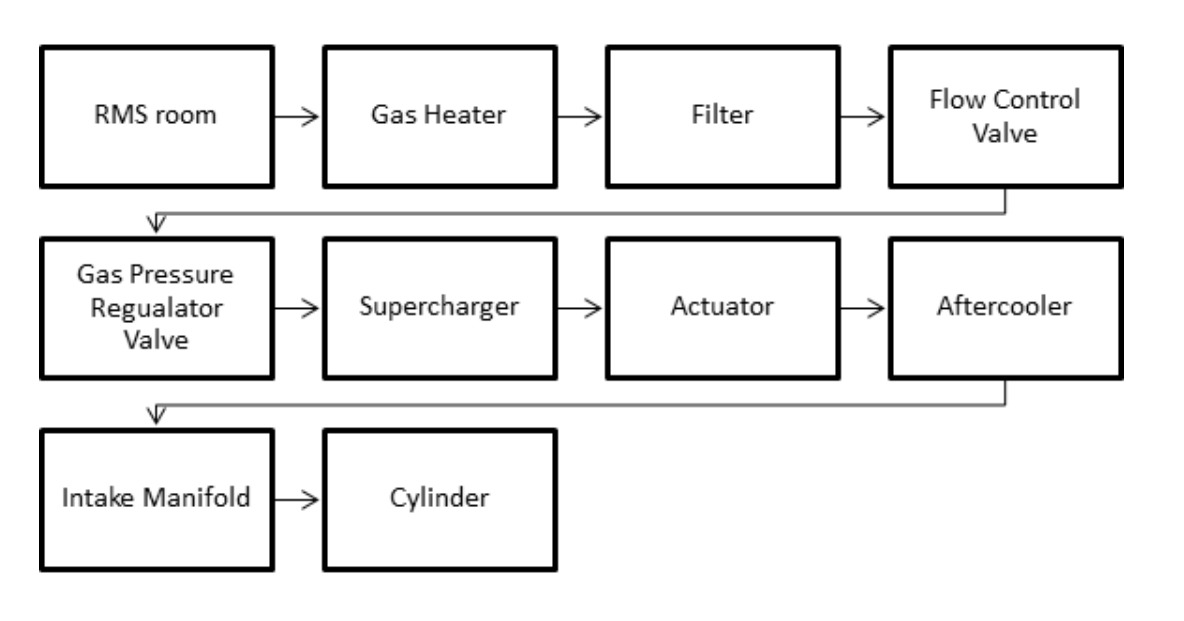
\includegraphics[width=0.98\linewidth]{img/fuel_supply.jpeg}
              \caption{Fuel Supply System}
            \end{center}
          \end{figure}


          The fuel filter is used to ensure clean fuel intake while the regulators are used to ensure proper gas pressure intake and accurate mixing process. 


          \subsection*{Ignition System}
          The ignition system provides a high energy spark to ignite the air/fuel mixture in the combustion chamber. It consists of the following components:
          \begin{itemize}
            \item The electronic ignition system
            \item The detonation sensing timing 
          \end{itemize}

          \begin{figure}[H]
            \begin{center}
              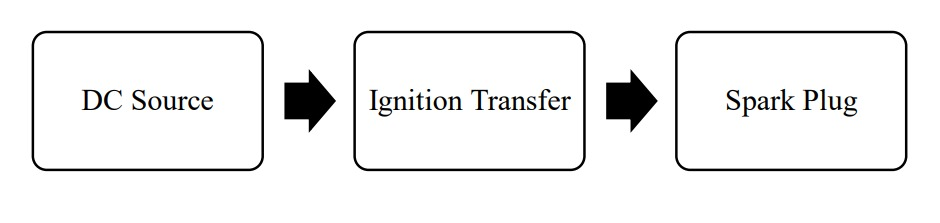
\includegraphics[width=0.8\linewidth]{img/ignition_system.jpeg}
              \caption{Ignition System in SI engine}
            \end{center}
          \end{figure}

          \subsection*{Cooling System}
          The primary purpose of the cooling system is to remove excess heat and hence maintain a safe temperature in the system so that all the components of the engine can function properly. It consists of the following components:
          \begin{itemize}
            \item Thermostats
            \item Jacket water pump
            \item After cooler water pump 
            \item After cooler Thermostats
            \item Housing 
          \end{itemize}

          \begin{figure}[H]
            \begin{center}
              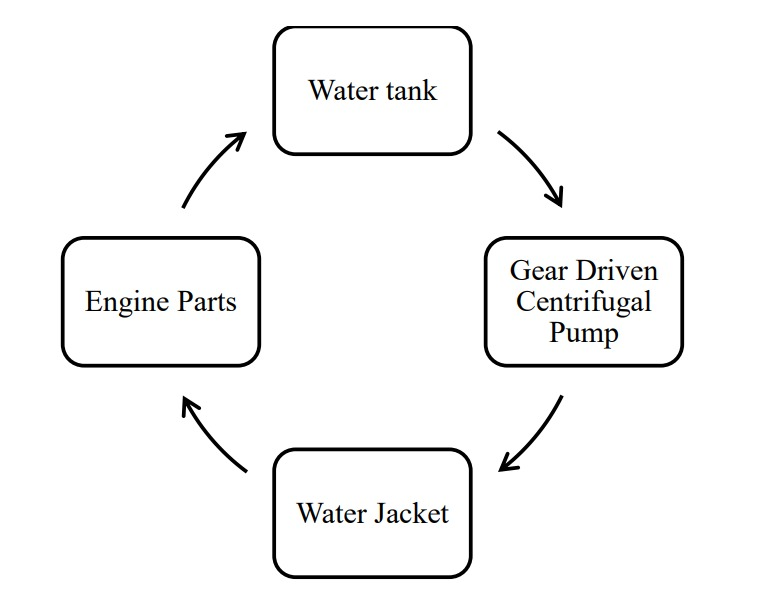
\includegraphics[width=0.5\linewidth]{img/ignition_si.jpeg}
              \caption{Cooling System in SI engine}
            \end{center}
          \end{figure}


          \subsection*{Lubrication System}
          The lubrication system provides a continuous supply of filtered oil to all the moving parts of the engine. It consists of the following components:
          \begin{itemize}
            \item Oil bypass filter removal 
            \item Oil pan 
            \item Sump pump 
            \item Air prelude pump 
            \item Lubricating oil
          \end{itemize}

          \begin{figure}[H]
            \begin{center}
              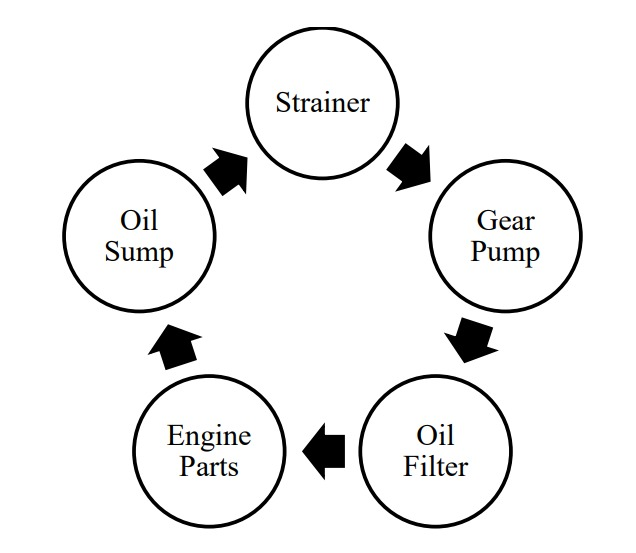
\includegraphics[width=0.5\linewidth]{img/lubrication.jpeg}
              \caption{Lubrication System}
            \end{center}
          \end{figure}

          The lubricating oil is used to reduce friction, heat and wear between the moving parts of the engine.

          \subsection*{Exhaust System}
          The exhaust system removes the exhaust gases from the engine. It consists of the following components:
          \begin{itemize}
            \item Water cooled exhaust manifold
            \item Flexible Fittings 
          \end{itemize}
          Water cooled exhaust manifold is used to cool the exhaust gases before they are released into the atmosphere.

          \begin{figure}[H]
            \begin{center}
              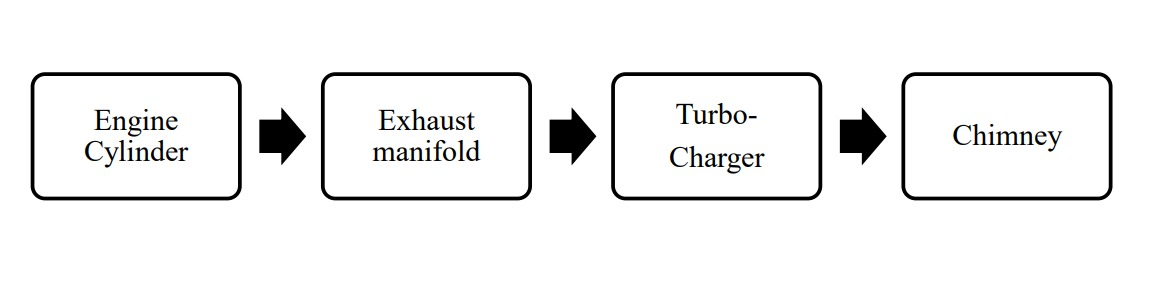
\includegraphics[width=0.9\linewidth]{img/exhaust_system.jpeg}
              \caption{Exhaust System}
            \end{center}
          \end{figure}

          \subsection*{Engine Protection System}
          The engine protection system monitors the engine and shuts it down if any of the conditions occur, like - rise in temperature or pressure, low oil pressure, low coolant level, etc. It consists of the following components:
          \begin{itemize}
            \item Electric Shutoff System 
            \item Gas Shutoff System
            \item Relief Valves 
            \item Wiring System 
          \end{itemize}

          \subsection*{Engine Control System}
          The engine control system controls the engine speed and monitors the engine operating conditions. It consists of the following components:
          \begin{itemize}
            \item Air-fuel Ratio Control 
            \item A3 Electronic Control Unit (ECU)
            \item Instrument Panel 
          \end{itemize}

          \subsection*{Power Distribution System}
          The power distribution system distributes the power generated by the engine to the load. The generators are operated in isochronous mode i.e. the supply frequency is kept constant. When load increases, frequency drops. The drop is sensed by governor and it increases fuel supply. When the 2 generators are operated simulataneously, they must be sysnchronized.

          There are 9 substations for distributing power: 
          \begin{multicols}{2}
            \begin{enumerate}
              \item Main Substation I 
              \item Main Substation II
              \item Main Substation III
              \item Dr. Rashid Hall Substation 
              \item Nazrul Islam Hall Substation [old]
              \item Nazrul Islam Hall Substation [new]
              \item New Academic Building Substation I 
              \item New Academic Building Substation II
              \item New Academic Building Substation III
            \end{enumerate}
          \end{multicols}

          \subsection*{Data Sheet}
          \begin{figure}[H]
            \begin{center}
              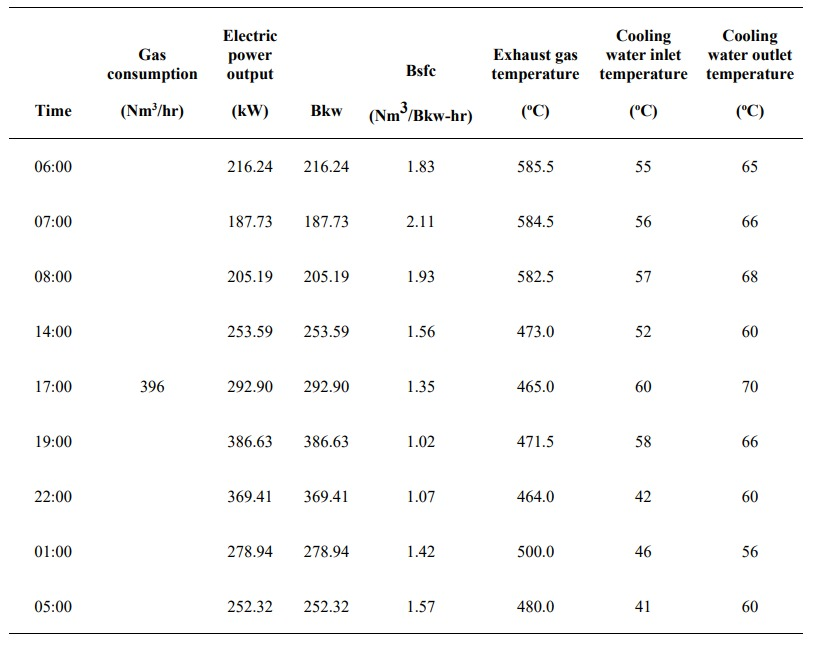
\includegraphics[width=0.98\linewidth]{img/data_table.jpeg}
            \end{center}
          \end{figure}
          \begin{center}
            \textbf{Table 3:} Performance data of the engines at various times of the day. 
          \end{center}

          \subsection*{Sample Calculation}
          For obseration no : 5 \\
          Time: 17:00 hr \\
          Gas consumption = 396 $Nm^3/hr$ \\
          Electric Power Output = Bkw = 292.90 kW \\

          $\therefore$ Bsfc = $\frac{\text{Gas consumption}}{Bkw}$  = 396/292.90 = 1.35 $Nm^3/kW-hr$ \\ 


          \subsection*{Graph}
          \begin{figure}[H]
            \begin{center}
              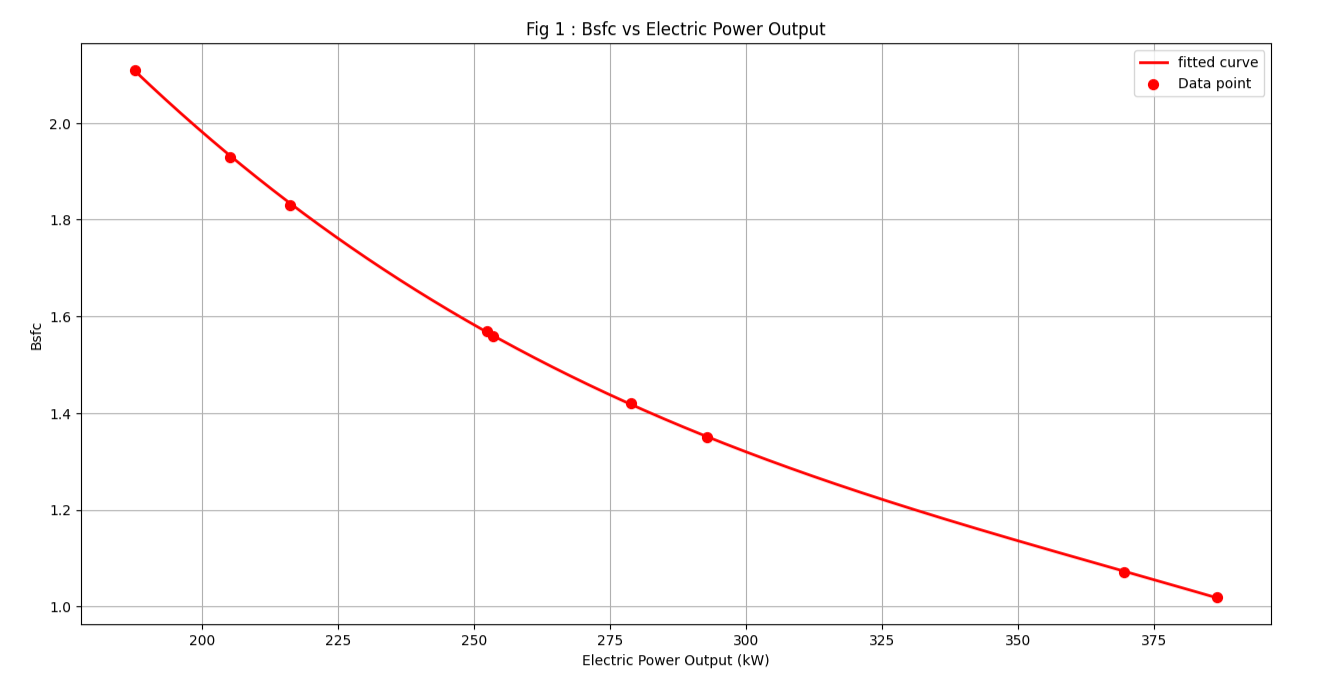
\includegraphics[width=0.99\linewidth]{img/Figure_1.png}
              \textbf{Bsfc vs Electric Output Power}
            \end{center}
          \end{figure}

          \begin{figure}[H]
            \begin{center}
              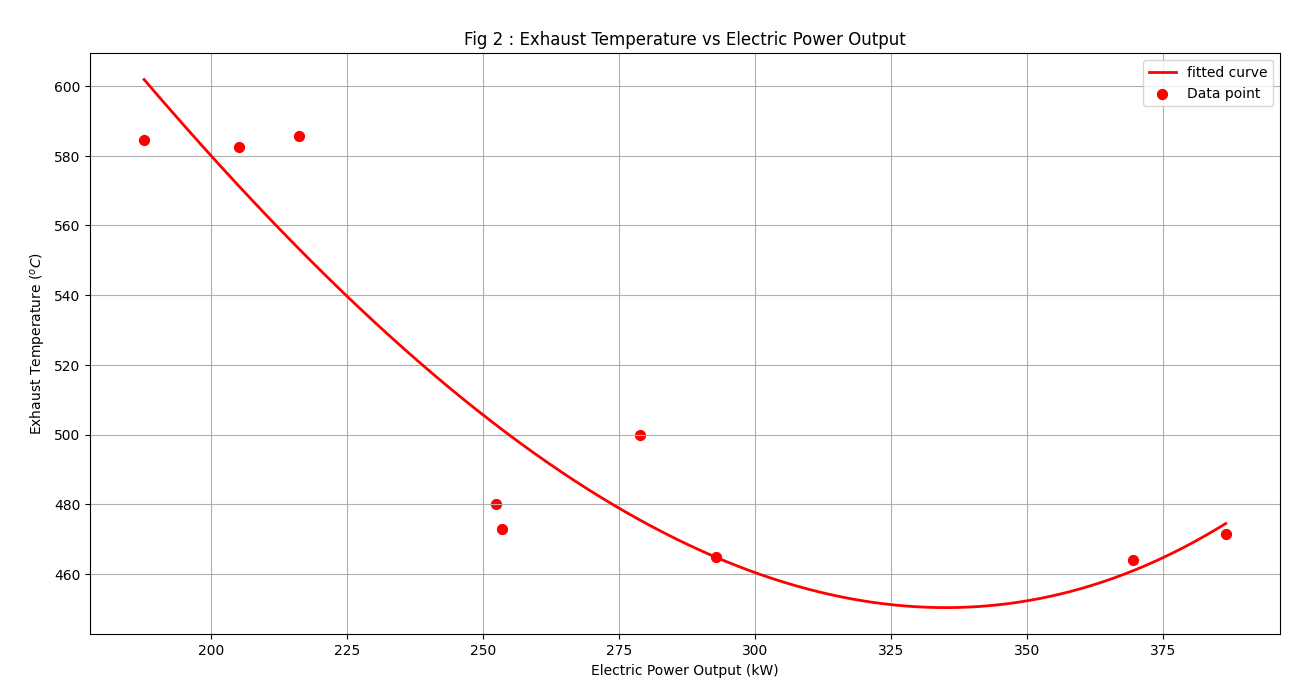
\includegraphics[width=0.99\linewidth]{img/Figure_2.png}
              \textbf{Exhaust Gas Temperature vs Electric Output Power}
            \end{center}
          \end{figure}

          \subsection*{Discussion}
          In this experiment, we went to the BUET power plant, which is on the BUET west campus. It can produce 5MW of electricity using three units: one that can make 1MW and two that can make 2MW each. These units all use engines that run on gas.\\

          When they start the engine, they check the level of lubricating oil. They also manually increase the oil pressure to make sure it reaches all parts of the engine. There's a 24V DC power source that provides electricity to the engine before it connects to the generator.\\

          Under the generator, there are springs to help absorb shock. There are pipes: a blue one for cool water going in and a red one for hot water coming out of the engine. The power plant has a cooling tower. The two 2MW units use a forced draft fan, while the 1MW unit uses an induced draft fan in the cooling tower.\\

          The engine is never pushed beyond 80\% of its capacity to make it last longer. Running it at full power would harm both the engine and the power plant.\\

          Normally, when an engine produces more power, its exhaust gas gets hotter. But in this case, looking at a graph of exhaust gas temperature versus power, we see that the temperature actually goes down as power increases. The graph isn't perfect because the power didn't change smoothly over time, causing the temperature to change unevenly.\\

          Another graph shows that as the power produced by the engine (Bkw) goes up, the fuel consumption (Bsfc) goes down. However, after a certain point, Bsfc starts to increase again. This is a common behavior in internal combustion engines.\\

          In general, the BUET power plant supplies electricity to teachers' homes, student halls, and academic buildings. This experiment was important for understanding how power plants are built and run. It helped us visualize what we learned from books to real-life situations. 
\end{document}
